% -- Exemplo Prático
\chapter{Exemplo prático}

\section{Primeira aplicação - Contatos}

Crie uma nova aplicação chamada \textbf{Contatos}. Para o nome do pacote use \inlinecode{contatos.app}.
Chame a \texttt{Activity} de \texttt{MainActivity}, que será responsável pela Atividade Principal. Depois
configure a plataforma Android a ser utilizada e \texttt{Finish} (em caso de dúvida verifique o item
\ref{sssec:testando} Testando o ADT).

Essa pode não ser uma aplicação muito útil, mas com ela poderemos aprender como funciona o Android. Você
só poderá criar algo se você souber utilizar as ferramentas.

\subsection{AndroidManifest.xml}

Esse é o arquivo que define nossa aplicação, mapeia as \texttt{Activity}'s, entre outras configurações. Ao finalizar
a criação do projeto, inicialmente este arquivo deverá conter o seguinte conteúdo:

% AndroidManifest.xml
\begin{listing}[H]
  \inputminted[linenos=true,frame=bottomline,tabsize=3]{ xml }{ source/AndroidManifest-1.xml }
  \caption{Projeto inicial [AndroidManifest.xml]}
\end{listing}

\subsection{Activity\label{ssec:act}}

Não existe método \inlinecode{main} visível ao programador no Android. Ao invés disso temos \texttt{Activity}'s.
Para que o Android saiba qual ele deve iniciar primeiro utilizamos um \texttt{intent-filter} como visto
no trecho de código acima da linha \circled{09} a \circled{12}.
Para nossa primeira \texttt{Activity} criaremos uma lista de contatos e um menu para criação de novo contato.

Para construir o layout inicial de nossa aplicação precisamos editar o arquivo \texttt{main.xml} localizado em
\texttt{res/layout}.

% res/layout/main.xml
\begin{listing}[H]
  \inputminted[linenos=true,frame=bottomline,tabsize=3]{ xml }{ source/main-1.xml }
  \caption{Layout principal [res/layout/main.xml]}
\end{listing}

Deste momento em diante tenha em mente que os arquivos \texttt{\gls{xml}} aqui descritos são apenas para
você poder comparar e ver se não esqueceu nada. Todos os \textit{layout}'s devem ser criados usando a
ferramenta ADT. Você irá notar que ao abrir o \texttt{xml} uma janela de \textit{layout} aparecerá.
Para visualizar o \texttt{xml} ou o \textit{layout} gráfico basta utilizar a aba inferior esquerda.

Por fim, temos o menu. Clique com o botão direito do \textit{mouse} em seu projeto e \texttt{New
$\rightarrow$ Other...} ou \texttt{Ctrl + N}. Procure por \texttt{Android XML File}. Em \texttt{Resource
Type} escolha a opção \texttt{Menu}. Chame-o de \texttt{main\b{ }menu.xml}.

% res/menu/main_menu.xml
\begin{listing}[H]
  \inputminted[linenos=true,frame=bottomline,tabsize=3]{ xml }{ source/main_menu-1.xml }
  \caption{Menu principal [res/menu/main\b{ }menu.xml]}
\end{listing}

Pronto, já temos nosso layout. Compile o projeto e vamos a próxima iteração.

\subsubsection{Convenção de nomes para ícones\label{sssec:nomeicones}}

Observe que o ícone utilizado no menu vem junto com o SDK do Android. Você pode visualizar os
ícones em \texttt{SDK\b{ }INSTALL/plataforms/android-8/data/res/drawable-hdpi}
(substitua \texttt{SDK\b{ }INSTALL} pelo diretório de instalação do SDK do Android, no nosso caso
\texttt{usr/local/lib/android-sdk}, \ref{ssec:sdk}). Note que há \textit{namespaces} ou prefixos em
cada um dos ícones. O Android recomenda a seguinte convenção:

\begin{table}[H]
\begin{tabularx}{440pt}{lXX}
\hline
\textbf{Tipo de Recurso} & \textbf{Prefixo} & \textbf{Exemplo} \\
\hline
Ícones & \texttt{ic\b{ }} & \texttt{ic\b{ }adicionar.png}\\
Launcher icons & \texttt{ic\b{ }launcher\b{ }} & \texttt{ic\b{ }launcher\b{ }calendario.png}\\
Menu e Action Bar & \texttt{ic\b{ }menu\b{ }} & \texttt{ic\b{ }menu\b{ }ajuda.png}\\
Status bar icons & \texttt{ic\b{ }stat\b{ }notify\b{ }} & \texttt{ic\b{ }stat\b{ }notify\b{ }msg.png}\\
Tab icons & \texttt{ic\b{ }tab\b{ }} & \texttt{ic\b{ }tab\b{ }recente.png}\\
Dialog icons & \texttt{ic\b{ }dialog\b{ }} & \texttt{ic\b{ }dialog\b{ }info.png}\\
\hline
\end{tabularx}
\caption{Convenção para nome dos ícones}
\end{table}

Note que você não é obrigado a utilizar os prefixos citados acima, isto é apenas uma convenção.
Veja mais detalhes em \url{http://developer.android.com/guide/practices/ui_guidelines/icon_design.html}.

Abra o arquivo \texttt{MainActivity.java} e vá ao método \inlinecode{onCreate}. Defina o \textit{layout} como
sendo nosso \texttt{main.xml}. Para isso adicione o \textit{layout} \textbf{main} ao final do método:

% MainActivity.java
\begin{listing}[H]
  \inputminted[linenos=true,frame=bottomline,tabsize=3]{ java }{ source/MainActivity-1.java }
  \caption{Definir layout [MainActivity.java]}
\end{listing}

\paragraph{Cuidado:\label{par:r}} no ambiente Android temos uma classe chamada \texttt{R}. Ela existe tanto
na biblioteca do Android como em cada projeto. Nesse caso faça o \textit{import} da classe
\texttt{contatos.app.R}. A classe \texttt{android.R} é utilizada em outras situações, onde códigos
pré-prontos foram disponibilizados pela equipe do Android.

Agora precisamos sobrescrever os métodos \inlinecode{onCreateOptionsMenu} e \inlinecode{onOptionsItemSelected}.
Eles irão criar o menu a partir de nosso \textit{layout} e notificar quando os itens do menu forem
pressionados, respectivamente. Vamos ao código:

% MainActivity.java
\begin{listing}[H]
  \inputminted[linenos=true,frame=bottomline,tabsize=3]{ java }{ source/MainActivity-2.java }
  \caption{Criando o menu [MainActivity.java]}
\end{listing}

\subsection{Formulários}

Agora vamos criar nosso formulário para criação e edição de contatos. Começaremos pelo \textit{layout}.
Crie um arquivo \texttt{xml} em \texttt{res/layout} chamado \texttt{salvar.xml}.

Existem alguns pontos importantes para este trecho de código. Começando pelo \textit{layout} inicial,
onde usaremos \texttt{TableLayout}. Esse \textit{layout} é ideal para telas com estilo tabela.

Um detalhe importante para observarmos neste \textit{layout} é que ele possui o atributo
\texttt{stretchColumns} com valor \texttt{1}. Isso quer dizer que a coluna \texttt{1} da tabela
terá o maior tamanho possível, respeitando o tamanho mínimo das outras células. Para visualizar as mudanças
você pode tentar usar outros valores como \texttt{0} tornando a primeira coluna maior que as demais,
ou ainda \texttt{*} que fará com que todas as células tenham o mesmo tamanho.

% res/layout/salvar.xml
\begin{listing}[H]
  \inputminted[linenos=true,frame=bottomline,tabsize=3]{ xml }{ source/salvar-1.xml }
  \caption{Formulário principal [res/layout/salvar.xml]}
\end{listing}

Crie uma nova \texttt{Activity} chamada \texttt{SalvarActivity} dentro de \texttt{contatos.app.view}.
Para irmos de uma \texttt{Activity} para outra precisamos de um \texttt{Intent}. Um de seus construtores recebe
como parâmetros a instância da classe em que estamos, sendo que ela deve implementar a interface \texttt{Context}
e o nome da classe a qual deve ser mostrada. Veja como implementar o método \inlinecode{irParaSalvar}
da classe \texttt{MainActivity}:

% MainActivity.java
\begin{listing}[H]
  \inputminted[linenos=true,frame=bottomline,tabsize=3]{ java }{ source/MainActivity-3.java }
  \caption{Mudando de Activity [MainActivity.java]}
\end{listing}

Veremos agora como manipular \texttt{EditText}'s, que representam os campos de entrada de dados. Abra o
\texttt{SalvarActivity} e adicione o método \inlinecode{carregar} e crie atributos para guardar os \texttt{EditText}'s:

% SaveActivity.java
\begin{listing}[H]
  \inputminted[linenos=true,frame=bottomline,tabsize=3]{ java }{ source/SalvarActivity-1.java }
  \caption{Utilizando EditText's [SalvarActivity.java]}
\end{listing}

Para que a \texttt{Activity} funcione precisamos mapeá-la no arquivo \texttt{AndroidManifest.xml}. Adicione o
conteúdo abaixo entre as \textit{tags} \texttt{application}:

% AndroidManifest.xml
\begin{listing}[H]
  \inputminted[linenos=true,frame=bottomline,tabsize=3]{ xml }{ source/AndroidManifest-2.xml }
  \caption{Mapear SalvarActivity [AndroidManifest.xml]}
\end{listing}

Utilize sempre o ADT e apenas confira se o arquivo está da maneira correta.

\subsection{Construindo o Model da aplicação\label{ssec:model}}

Precisamos de um \textit{helper} para fazer acesso ao banco de dados. O Android provê suporte
a bancos de dados Sqlite por padrão. Qualquer banco de dados que você criar será acessível pelo nome
por qualquer classe na sua aplicação, mas não fora dela.

Crie uma classe chamada \texttt{ContatoHelper} em \texttt{contatos.app.model} que extende de
\texttt{SQLiteOpenHelper}. Essa classe será capaz de ler e escrever no banco de dados graças aos métodos 
\inlinecode{getReadableDatabase()} e \inlinecode{getWritableDatabase()}, respectivamente.

A princípio temos que criar um construtor passando como parâmetros o nome do banco de dados e a versão
da \gls{ddl}. Logo em seguida precisamos implementar os métodos \inlinecode{onCreate}, no qual iremos
criar as tabelas e \inlinecode{onUpdate}, caso tenhamos que alterar alguma tabela.

% ContatoHelper.java
\begin{listing}[H]
  \inputminted[linenos=true,frame=bottomline,tabsize=3]{ java }{ source/ContatoHelper-1.java }
  \caption{Helper da aplicação [ContatoHelper.java]}
\end{listing}

Para a iteração de criação de um novo contato, ainda em \texttt{ContatoHelper} vamos adicionar um método
\inlinecode{criar}. Faça:

% ContatoHelper.java
\begin{listing}[H]
  \inputminted[linenos=true,frame=bottomline,tabsize=3]{ java }{ source/ContatoHelper-2.java }
  \caption{Criar novo contato [ContatoHelper.java]}
\end{listing}

Agora temos que fazer a chamada do método \inlinecode{criar} da classe \texttt{ContatoHelper} em
\texttt{SalvarActivity}. Para isso temos que criar uma instância de \texttt{ContatoHelper}, adicionar
o botão salvar e adicionar um \textit{Listener} de \textit{click} (faça o \textit{import}
da classe\\ \texttt{android.view.View.OnClickListener}). Vamos ao código:

% SaveActivity.java
\begin{listing}[H]
  \inputminted[linenos=true,frame=bottomline,tabsize=3]{ java }{ source/SalvarActivity-2.java }
  \caption{Fim da iteração criar contato [SalvarActivity.java]}
\end{listing}

Com essa implementação já é possível salvar contatos na base de dados.

\subsection{Mostrando os dados na View\label{ssec:listview}}

Após salvar os dados no banco, devemos ser capazes de obter tais informações e colocá-las em forma
de Lista. Para isso criaremos um novo \textit{layout} que será responsável por representar uma linha
de nossa Lista. Essa linha deve ser semelhante a figura abaixo:

\begin{figure}[h]
\centering
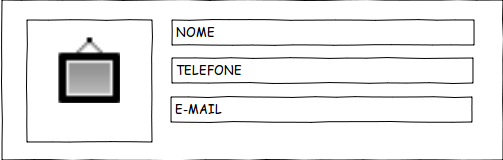
\includegraphics[scale=0.6]{img/layout-linha.png}
\caption{Layout linha da Lista}
\end{figure}

Para isso crie um arquivo chamado \texttt{linha.xml} em \texttt{res/layout} com o seguinte conteúdo.
% -- TODO: exemplificar o trecho de código.

% res/layout/linha.xml
\begin{listing}[H]
  \inputminted[linenos=true,frame=bottomline,tabsize=3]{ xml }{ source/linha-1.xml }
  \caption{Layout para cada linha da lista [res/layout/linha.xml]}
\end{listing}

Agora vamos até \texttt{ContatoHelper} e adicionar o método \inlinecode{listar}. E também adicionaremos
métodos para facilitar obter os valores de cada atributo.

% ContatoHelper.java
\begin{listing}[H]
  \inputminted[linenos=true,frame=bottomline,tabsize=3]{ java }{ source/ContatoHelper-3.java }
  \caption{Listar contatos existentes [ContatoHelper.java]}
\end{listing}

Para popular cada linha de nossa Lista vamos criar uma classe interna (\textit{inner class}) em
\texttt{MainActivity}. Assim podemos fazer \textit{cache} dos objetos aumentando a performance.
Use o sufixo \texttt{Holder} para esse tipo de classe.

% MainActivity.java
\begin{listing}[H]
  \inputminted[linenos=true,frame=bottomline,tabsize=3]{ java }{ source/MainActivity-4.java }
  \caption{Classe Holder [MainActivity.java]}
\end{listing}

Levando em conta que estamos usando a interface \texttt{Cursor} em nosso \texttt{Helper} temos
que criar uma classe que extende de \texttt{CursorAdapter} que será responsável por definir o
\textit{layout} de cada linha da Lista. Crie uma classe interna chamada \texttt{ContatoAdapter}.
Iremos sobrescrever dois métodos, \inlinecode{newView()} e \inlinecode{bindView()}, que são responsáveis
por inflar (\textit{inflate}) uma nova linha e reciclar uma linha existente, respectivamente.

% MainActivity.java
\begin{listing}[H]
  \inputminted[linenos=true,frame=bottomline,tabsize=3]{ java }{ source/MainActivity-5.java }
  \caption{Classe Adapter [MainActivity.java]}
\end{listing}

Com a introdução do \texttt{Helper} teremos que criar uma instância da classe \texttt{Cursor}
para popular nossa \texttt{ListView}. Vamos ao código-fonte:

% MainActivity.java
\begin{listing}[H]
  \inputminted[linenos=true,frame=bottomline,tabsize=3]{ java }{ source/MainActivity-6.java }
  \caption{Popular ListView [MainActivity.java]}
\end{listing}

Nunca esquecendo de fechar o \texttt{helper} ao sair, pois assim garantimos que a conexão com
o banco será fechada.

\subsection{Editando dados existentes}

Para a edição de informações usaremos o mesmo \texttt{Activity} do criar, ou seja, \texttt{SalvarActivity}.
Para isso precisamos passar um parâmetro para o \texttt{Activity}. Usaremos então um método do
\texttt{Intent} que é responsável por isso, \inlinecode{putExtra(chave, valor)}.

Para uma passagem de parâmetros segura devemos usar um \textit{namespace} para que não colida com
nenhum nome já utilizado pelo Android. Para isso criaremos uma variável estática do tipo \texttt{String}.
Isso acontecerá quando o usuário pressionar a linha que ele deseja editar. Podemos fazer isso utilizando
a interface \texttt{OnItemClickListener}.

Vamos incrementar também o método \inlinecode{irParaSalvar} passando o parâmetro caso haja um. Vamos ao
código:

% MainActivity.java
\begin{listing}[H]
  \inputminted[linenos=true,frame=bottomline,tabsize=3]{ java }{ source/MainActivity-7.java }
  \caption{Passagem de parâmetros [MainActivity.java]}
\end{listing}

Agora é hora de tratar nosso parâmetro no \texttt{SalvarActivity}. Caso haja um parâmetro precisamos
obter os dados existentes no banco de dados para então editá-lo. Neste caso precisaremos de mais dois
métodos em \texttt{ContatoHelper}, que são \inlinecode{ler} e \inlinecode{atualizar}.

% ContatoHelper.java
\begin{listing}[H]
  \inputminted[linenos=true,frame=bottomline,tabsize=3]{ java }{ source/ContatoHelper-4.java }
  \caption{Ler e atualizar dados existentes [ContatoHelper.java]}
\end{listing}

O próximo passo é tratar no \texttt{SalvarActivity} caso o parâmetro tenha sido enviado ou não. Caso positivo
devemos carregar os dados existentes no banco de dados e depois atualizá-los.

% SaveActivity.java
\begin{listing}[H]
  \inputminted[linenos=true,frame=bottomline,tabsize=3]{ java }{ source/SalvarActivity-3.java }
  \caption{Usando Activity para criar ou atualizar [SalvarActivity.java]}
\end{listing}
